\chapter{Ciclos biogeoquímicos}\label{ch:b2:biogeochemical-cycles}

Em março de 1958, um jovem químico chamado Charles Keeling ligou um
analisador de gás por infravermelho na encosta norte do Mauna Loa, no
Havaí, três quilômetros e meio acima do Pacífico, onde o ar é tão bem
misturado quanto o ar pode ser. Ele esperava medir uma constante; em um
ano, tinha um dente de serra --- o dióxido de carbono subindo a cada
inverno e descendo a cada verão, à medida que as florestas do hemisfério
norte expiravam e inspiravam --- e, em poucos anos, uma inclinação sob o
dente de serra que não parou desde então. A \omterm{prop:b2:biogeochemical-cycles:carbon}{curva de Keeling} é a
respiração da biosfera vista de fora, com um gráfico de febre desenhado
por cima. Este capítulo trata dos ciclos que a curva registra: onde o
carbono, o nitrogênio, o fósforo e o enxofre dos seres vivos estão
armazenados, com que rapidez eles se movem entre \omterm{def:b2:biogeochemical-cycles:reservoir}{reservatórios}, o que
fixa essas velocidades --- em sua maioria, os metabolismos do
\cref{ch:b2:microbial-metabolism} --- e o que uma única espécie fez com
cada ciclo em duzentos anos.

\section{Reservatórios, fluxos e tempos de residência}

\begin{definition}[Reservatório, fluxo, tempo de residência]\label{def:b2:biogeochemical-cycles:reservoir}
\index{reservatório}\index{fluxo}\index{tempo de residência}\index{estado estacionário}\index{ciclo biogeoquímico}
Um \emph{ciclo biogeoquímico} é o movimento de um elemento entre
\emph{reservatórios} (a atmosfera, o oceano, os solos, a biomassa viva,
as rochas) por meio de \emph{fluxos} medidos em massa por ano. Um
reservatório de massa $M$ com saída total $F$ tem um \emph{tempo de
residência} $\tau = M/F$, o tempo médio que um átomo passa nele; em
\emph{estado estacionário}, a entrada é igual à saída e $M$ é constante.
Os ciclos são acoplados pela estequiometria da vida --- a
\emph{razão de Redfield} do plâncton marinho, $\mathrm{C:N:P} =
106:16:1$ em átomos ---, de modo que o suprimento do elemento mais escasso
fixa a taxa com que todos os outros são absorvidos.
\end{definition}

\begin{theorem}[O modelo de uma caixa]\label{thm:b2:biogeochemical-cycles:box}
\index{modelo de caixa}\index{tempo de relaxação}
Se um \omterm{def:b2:biogeochemical-cycles:reservoir}{reservatório} perde seu conteúdo a uma taxa proporcional ao que
contém, $F_{\text{sai}} = M/\tau$, e recebe uma entrada constante
$F_{\text{ent}}$, então
\[
\frac{\mathrm{d}M}{\mathrm{d}t} = F_{\text{ent}} - \frac{M}{\tau},
\qquad
M(t) = M^{*} + (M_0 - M^{*})\,e^{-t/\tau}, \qquad M^{*} = F_{\text{ent}}\tau :
\]
o \omterm{def:b2:biogeochemical-cycles:reservoir}{reservatório} relaxa para um \omterm{def:b2:biogeochemical-cycles:reservoir}{estado estacionário} proporcional à sua
entrada, com o \omterm{def:b2:biogeochemical-cycles:reservoir}{tempo de residência} como constante de tempo. Um aumento
em degrau da entrada eleva proporcionalmente o \omterm{def:b2:biogeochemical-cycles:reservoir}{estado estacionário}, e o
\omterm{def:b2:biogeochemical-cycles:reservoir}{reservatório} o acompanha em alguns $\tau$: um compartimento com \omterm{def:b2:biogeochemical-cycles:reservoir}{tempo de
residência} de dias (a amônia atmosférica, o nitrato de um lago na
primavera) acompanha suas fontes; um com \omterm{def:b2:biogeochemical-cycles:reservoir}{tempo de residência} de séculos
(o carbono do oceano profundo, a matéria orgânica do solo) as integra, e
a perturbação de um compartimento lento sobrevive à perturbação que a
causou.
\end{theorem}
\begin{proof}
A equação é linear com coeficientes constantes: o \omterm{def:b2:biogeochemical-cycles:reservoir}{estado estacionário}
$M^{*}$ anula o lado direito, e o desvio $m = M - M^{*}$ obedece a
$\dot m = -m/\tau$, logo $m = m_0 e^{-t/\tau}$. Se um \omterm{def:b2:biogeochemical-cycles:reservoir}{reservatório} tem
várias saídas, $\tau$ é fixado pela soma delas, $1/\tau = \sum_i
1/\tau_i$: o sumidouro mais rápido domina.
\end{proof}

\section{O ciclo do carbono}

\begin{proposition}[O balanço de carbono]\label{prop:b2:biogeochemical-cycles:carbon}
\index{ciclo do carbono}\index{fração atmosférica}\index{sumidouro de carbono}\index{curva de Keeling}
Em gigatoneladas de carbono (\unit{GtC}, $10^{12}$~kg), os principais
\omterm{def:b2:biogeochemical-cycles:reservoir}{reservatórios} são a atmosfera (cerca de 880 nos anos 2020, 590 antes da
indústria), as plantas terrestres (450), os solos (1700), o oceano
superficial (900), o oceano profundo (\num{37000}) e as rochas
sedimentares (\num{e8}); os combustíveis fósseis são a fração destas
últimas que a indústria consegue alcançar, cerca de \num{5000}. Os
\omterm{def:b2:biogeochemical-cycles:reservoir}{fluxos} naturais são grandes e quase equilibrados: a fotossíntese em
terra retira cerca de 120 por ano, e a respiração e a decomposição os
devolvem; a superfície do oceano troca cerca de 80 em cada sentido com o
ar. O \omterm{def:b2:biogeochemical-cycles:reservoir}{fluxo} humano é pequeno diante desses --- cerca de 10 por ano dos
combustíveis fósseis e 1 do desmatamento ---, mas tem sentido único, e a
atmosfera reteve \emph{cerca de \qty{45}{\%}} dele (a \emph{\omterm{prop:b2:biogeochemical-cycles:carbon}{fração
atmosférica}}), com o oceano absorvendo um quarto e a terra, fertilizada
pelo $\mathrm{CO_2}$ adicional, o restante. Uma parte por milhão de $\mathrm{CO_2}$ atmosférico
equivale a \qty{2.13}{GtC}; a concentração subiu de 280 para \num{315}~ppm
entre 1750 e 1958, e de 315 para mais de \num{420} entre 1958 e os anos
2020, atualmente a \qty{2.5}{ppm} por ano. O \omterm{def:b2:biogeochemical-cycles:reservoir}{tempo de residência} de uma
molécula de $\mathrm{CO_2}$ no ar, $880/200 \approx 4$ anos,
é curto; o tempo de vida do \emph{excesso}, fixado pela lenta mistura
com o oceano profundo e pelo intemperismo ainda mais lento das rochas, é
de séculos a milênios --- um quinto do que é emitido hoje ainda estará
no ar daqui a dez mil anos.
\end{proposition}
\begin{proof}[Evidências]
Três assinaturas mostram que o carbono acrescentado é fóssil. Seus
isótopos: o carbono fóssil não tem $\mathrm{{}^{14}C}$ (ele decaiu há
milhões de anos) e é empobrecido em $\mathrm{{}^{13}C}$, como todo carbono
vegetal, e a atmosfera vem perdendo ambos --- o efeito Suess, medido
nos anéis das árvores desde os anos 1950. Seu oxigênio: o
$\mathrm{O_2}$ da atmosfera cai no mesmo ritmo, segundo a estequiometria da
combustão, como mostrou o filho de Keeling nos anos 1990, o que uma fonte
vulcânica ou oceânica não produziria. Sua contabilidade: a soma do
carvão, do petróleo e do gás vendidos, convertida em carbono, excede o
aumento no ar por um fator de dois, e a metade que falta é encontrada no
carbono inorgânico dissolvido crescente e no pH decrescente do oceano, e
no sumidouro terrestre. O dente de serra sazonal, maior em Barrow, no
Alasca, que no Mauna Loa e quase ausente no polo Sul, é a absorção
estival e a liberação invernal das florestas do norte --- uma medida
direta da respiração da biosfera.
\end{proof}

\begin{omfigure}
\begin{tikzpicture}
\begin{axis}[
  width=0.9\linewidth, height=6cm,
  axis x line=bottom, axis y line=left,
  xmin=1955, xmax=2026, ymin=300, ymax=430,
  xlabel={ano}, ylabel={$\mathrm{CO_2}$ (ppm), média anual em Mauna Loa},
  xlabel style={font=\small, at={(axis description cs:0.5,-0.13)}, anchor=north},
  ylabel style={font=\small},
  tick label style={font=\small}, xtick={1960,1970,1980,1990,2000,2010,2020}, ytick={300,325,350,375,400,425},
  scaled x ticks=false, x tick label style={/pgf/number format/1000 sep=},
  clip=false,
]
\addplot[very thick, omDef, mark=*, mark size=1pt] coordinates {
(1959,316.0) (1962,318.5) (1965,320.0) (1968,323.0) (1971,326.3) (1974,330.2) (1977,333.8) (1980,338.8) (1983,342.8) (1986,347.2) (1989,353.1) (1992,356.4) (1995,360.8) (1998,366.7) (2001,371.1) (2004,377.5) (2007,383.8) (2010,389.9) (2013,396.5) (2016,404.2) (2019,411.4) (2022,418.5) (2024,424.6)};
\node[font=\scriptsize, anchor=north west, align=left] at (axis cs:1958,425) {anos 1960: \qty{+0.9}{ppm/ano}\\anos 2010: \qty{+2.4}{ppm/ano}};
\node[font=\scriptsize, anchor=west, align=left] at (axis cs:1990,320) {nível pré-industrial: \qty{280}{ppm};\\a cada ano, um dente de serra de\\$\pm\qty{3}{ppm}$ se sobrepõe a esta linha};
\end{axis}
\end{tikzpicture}

{\small A \omterm{prop:b2:biogeochemical-cycles:carbon}{curva de Keeling}: média anual do dióxido de carbono no ar em
Mauna Loa desde 1959. A inclinação quase triplicou; o dente de serra
sazonal sobreposto, não visível nesta escala, é a fotossíntese estival
do hemisfério norte.}
\end{omfigure}

\begin{omfigure}
\begin{tikzpicture}[every node/.style={font=\scriptsize}, >=stealth, box/.style={draw, rounded corners, minimum width=2.2cm, minimum height=0.9cm, align=center, fill=#1}]
  \node[box=omDef!15] (atm) at (0,3) {atmosfera\\880};
  \node[box=omThm!15] (veg) at (-4.4,0.6) {plantas terrestres 450\\solos 1700};
  \node[box=omProp!15] (surf) at (4.4,0.6) {oceano superficial\\900};
  \node[box=omProp!25] (deep) at (4.4,-1.6) {oceano profundo\\37\,000};
  \node[box=gray!20] (rock) at (0,-1.6) {rochas e combustíveis fósseis\\$10^{8}$; acessíveis $\sim 5000$};
  \draw[->, thick] ([xshift=-2mm]atm.south west) -- node[above left, pos=0.45] {120 fotossíntese} ([xshift=-4mm]veg.north);
  \draw[->, thick] ([xshift=5mm]veg.north) -- ([xshift=-2mm]atm.south); \node[anchor=north east] at (-0.4,1.5) {119 respiração, fogo};
  \draw[->, thick] ([xshift=2mm]atm.south east) -- node[above right, pos=0.45] {80 dissolução} ([xshift=4mm]surf.north);
  \draw[->, thick] ([xshift=-5mm]surf.north) -- ([xshift=2mm]atm.south); \node[anchor=north west] at (0.4,1.5) {78 desgaseificação};
  \draw[<->, thick] (surf) -- node[right] {$\sim 100$ mistura, afundamento} (deep);
  \draw[->, very thick, omExo!80!black] (rock.north) -- node[left, align=right, pos=0.4] {10 fósseis\\ + 1 uso da terra} (atm.south);
  \node[align=left, anchor=west] at (7.0,3.2) {fluxos em \unit{GtC/ano},\\ estoques em \unit{GtC}\\[2pt] dos 11 emitidos:\\ 5 ficam no ar,\\ 3 vão para a terra,\\ 3 para o oceano};
\end{tikzpicture}

{\small O \omterm{prop:b2:biogeochemical-cycles:carbon}{ciclo do carbono} em números redondos. As trocas naturais são
dez vezes o \omterm{def:b2:biogeochemical-cycles:reservoir}{fluxo} humano, mas quase se anulam; o \omterm{def:b2:biogeochemical-cycles:reservoir}{fluxo} humano não se
anula.}
\end{omfigure}

\begin{omfigure}
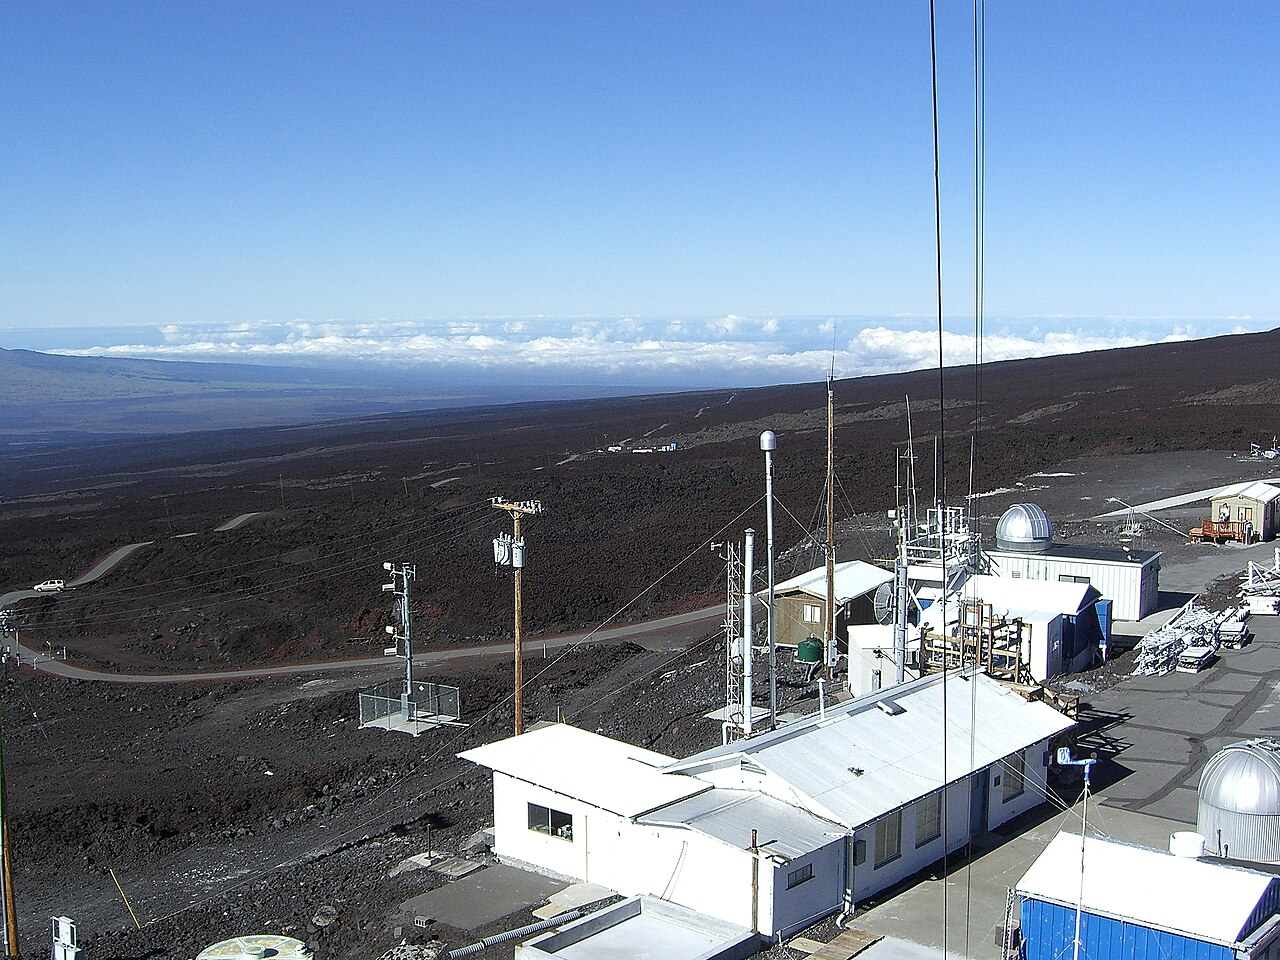
\includegraphics[width=0.56\linewidth]{images/book4/mauna-loa.jpg}\hspace{0.03\linewidth}
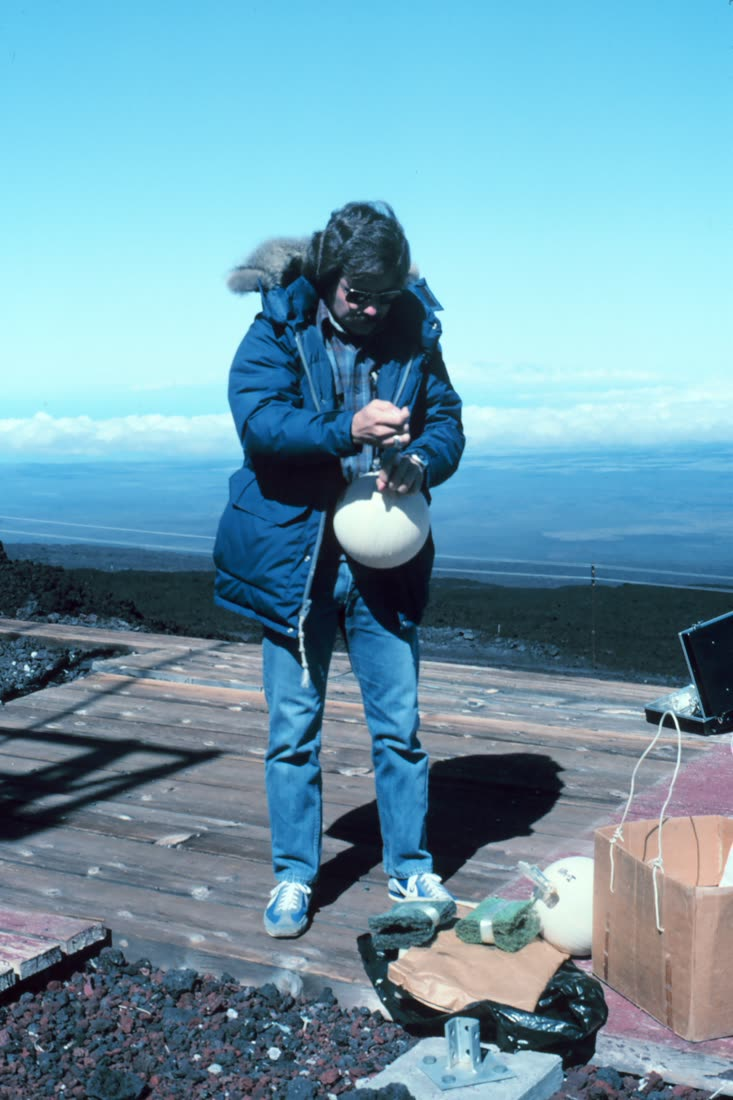
\includegraphics[width=0.33\linewidth]{images/book4/keeling-flask.jpg}

{\small Onde a curva é traçada. À esquerda: o observatório na encosta
norte do Mauna Loa, a \qty{3400}{m} de altitude, acima da inversão dos
alísios que mantém embaixo o próprio ar da ilha. À direita: uma amostra
em frasco sendo coletada em 1982; frascos como esses, analisados na
Califórnia, verificam o analisador contínuo e são enchidos em estações
que vão do Alasca ao polo Sul.}
\end{omfigure}

\section{O ciclo do nitrogênio}

\begin{proposition}[O ciclo do nitrogênio]\label{prop:b2:biogeochemical-cycles:nitrogen}
\index{ciclo do nitrogênio}\index{fixação de nitrogênio}\index{nitrificação}\index{desnitrificação}\index{processo Haber--Bosch}\index{anammox}
O nitrogênio é abundante --- o ar contém $4\times 10^{9}$~Tg de
$\mathrm{N_2}$ --- e escasso, porque a ligação tripla do $\mathrm{N_2}$ só é aberta
por dois processos: os raios (alguns Tg por ano) e a
\emph{fixação biológica de nitrogênio} por procariontes dotados de
nitrogenase, cerca de 100 Tg por ano em terra e 100 no mar, a um
custo de 16 ATP por $\mathrm{N_2}$. O nitrogênio fixado percorre então uma
escada redox movida por micróbios (\cref{ch:b2:microbial-metabolism}):
a \emph{amonificação} da matéria morta em $\mathrm{NH_4^{+}}$;
a \emph{nitrificação} do $\mathrm{NH_4^{+}}$ em $\mathrm{NO_2^{-}}$ e $\mathrm{NO_3^{-}}$ por
\omterm{def:b2:microbial-metabolism:trophic}{quimiolitotróficos} aeróbios; a absorção de $\mathrm{NH_4^{+}}$ ou $\mathrm{NO_3^{-}}$ pelas plantas
e sua redução de volta a amina; e, onde falta oxigênio, a
\emph{\omterm{def:b2:microbial-metabolism:anaerobic}{desnitrificação}} do $\mathrm{NO_3^{-}}$ em $\mathrm{N_2}$ (com um vazamento de $\mathrm{N_2O}$)
e o \emph{anammox}, a oxidação anaeróbia do amônio pelo
nitrito em $\mathrm{N_2}$, que juntos devolvem ao ar mais ou menos o que
a fixação retira. O \omterm{def:b2:biogeochemical-cycles:reservoir}{tempo de residência} de um átomo de nitrogênio na
biosfera é de algumas centenas de anos; na atmosfera, $4\times
10^{9}/400 \approx 10^{7}$ anos. Desde 1913, o processo
\emph{Haber--Bosch} fixa nitrogênio industrialmente, hoje cerca de 120
Tg por ano, e as leguminosas cultivadas e a queima de combustíveis
fósseis acrescentam 60 e 30: a atividade humana fixa tanto nitrogênio
quanto todos os processos naturais juntos, e alimenta metade das pessoas
vivas.
\end{proposition}

\begin{omfigure}
\begin{tikzpicture}[every node/.style={font=\scriptsize}, >=stealth, box/.style={draw, rounded corners, minimum width=1.9cm, minimum height=0.8cm, align=center, fill=#1}]
  \node[box=omDef!15] (n2) at (0,3.4) {$\mathrm{N_2}$ no ar\\$4\times 10^{9}$ Tg};
  \node[box=omThm!15] (org) at (-4.6,1.0) {N orgânico\\plantas, solos, mar};
  \node[box=omProp!15] (nh4) at (-2.2,-0.8) {$\mathrm{NH_4^{+}}$};
  \node[box=omProp!15] (no2) at (2.2,-0.8) {$\mathrm{NO_2^{-}}$};
  \node[box=omProp!15] (no3) at (4.6,1.0) {$\mathrm{NO_3^{-}}$};
  \draw[->, thick] (n2) -- node[above left, align=right] {fixação\\nitrogenase, 200\\Haber--Bosch 120} (org);
  \draw[->, thick] (org.south) -- node[below left] {amonificação} (nh4.north);
  \draw[->, thick] (nh4) -- node[below] {nitrificação} (no2);
  \draw[->, thick] (no2) -- node[below right] {nitrificação} (no3);
  \draw[->, thick] (no3) to[bend left=18] node[above, pos=0.72] {assimilação} (org);
  \draw[->, thick, omExo!80!black] (no3) -- node[above right, align=left] {desnitrificação\\(anóxica), vazamento de $\mathrm{N_2O}$} (n2);
  \draw[->, thick, omExo!80!black] (no2) -- node[right, pos=0.55, align=left] {anammox\\(com $\mathrm{NH_4^{+}}$)} (n2);
  \node[anchor=north, align=center] at (0,-1.5) {fluxos em Tg N por ano; todas as etapas, salvo assimilação e amonificação, são feitas por procariontes};
\end{tikzpicture}

{\small O \omterm{prop:b2:biogeochemical-cycles:nitrogen}{ciclo do nitrogênio} como escada redox (as plantas assimilam
tanto o amônio quanto o nitrato). A fixação e a \omterm{def:b2:microbial-metabolism:anaerobic}{desnitrificação}, as duas
portas para a atmosfera, são ambas microbianas; a porta industrial hoje
se iguala à natural.}
\end{omfigure}

\begin{proof}[Evidências]
Floresta Experimental de Hubbard Brook, em New Hampshire: em 1965, uma
bacia hidrográfica inteira foi desmatada por corte raso e mantida nua
com herbicida, enquanto uma vizinha foi deixada intacta, e os riachos que
drenavam cada uma foram medidos e analisados durante anos. A bacia
desmatada perdeu nitrato a sessenta vezes a taxa da testemunha --- todo o
capital de nitrogênio do solo, não mais absorvido pelas plantas, foi
nitrificado e lixiviado, levando consigo cálcio e potássio e acidificando
o riacho. O experimento mostrou quão fechado é o ciclo numa floresta
intacta (alguns quilogramas de nitrogênio perdidos por hectare por ano,
contra centenas reciclados) e o que o rompe.
\end{proof}

\section{Fósforo e enxofre}

\begin{proposition}[Dois ciclos sem gás rápido]\label{prop:b2:biogeochemical-cycles:ps}
\index{ciclo do fósforo}\index{ciclo do enxofre}\index{eutrofização}\index{sulfeto de dimetila}
O \emph{fósforo} não tem forma gasosa. Ele entra nos ecossistemas pelo
intemperismo da apatita das rochas, cerca de 20 Tg por ano sobre toda a
superfície terrestre, é reciclado nos solos e nos lagos muitas vezes
--- um íon fosfato na água superficial de um lago é absorvido em
horas --- e sai para os sedimentos, onde fica pelos
$10^{8}$ anos de um ciclo das rochas. A vida é, portanto, econômica em
fósforo e limitada pelo fósforo: o \omterm{def:b2:biogeochemical-cycles:reservoir}{tempo de residência} no oceano é de
cerca de \num{20000} anos, e o fosfato do mar profundo, trazido à
superfície pela ressurgência, fixa sua produtividade. A mineração
desloca hoje para as terras agrícolas mais ou menos tanto fósforo quanto
o intemperismo libera, e seu escoamento para os lagos causa a
\emph{eutrofização}: uma proliferação de algas, sua decomposição, o
consumo de oxigênio e a morte dos peixes --- os experimentos de
Schindler com lagos inteiros em Ontário, nos anos 1970, com uma metade de
um lago fertilizada com fósforo e a outra não, mostraram que só o fósforo
é o gatilho, e levaram à sua remoção dos detergentes. O \emph{enxofre}
tem ao mesmo tempo um ciclo das rochas (gipsita, pirita) e uma fase
gasosa: o $\mathrm{SO_2}$ dos vulcões e do carvão, o $\mathrm{H_2S}$ dos sedimentos
anóxicos e o \emph{\omterm{prop:b2:biogeochemical-cycles:ps}{sulfeto de dimetila}} do plâncton marinho, cujos
produtos de oxidação semeiam as nuvens sobre o oceano. A queima de
carvão triplicou o \omterm{def:b2:biogeochemical-cycles:reservoir}{fluxo} de enxofre para o ar no século XX e deu à
Europa e à América do Norte sua chuva ácida; os lavadores de gases a
reverteram em décadas, já que o \omterm{def:b2:biogeochemical-cycles:reservoir}{tempo de residência} do ciclo no ar é
de alguns dias.
\end{proposition}

\begin{omfigure}
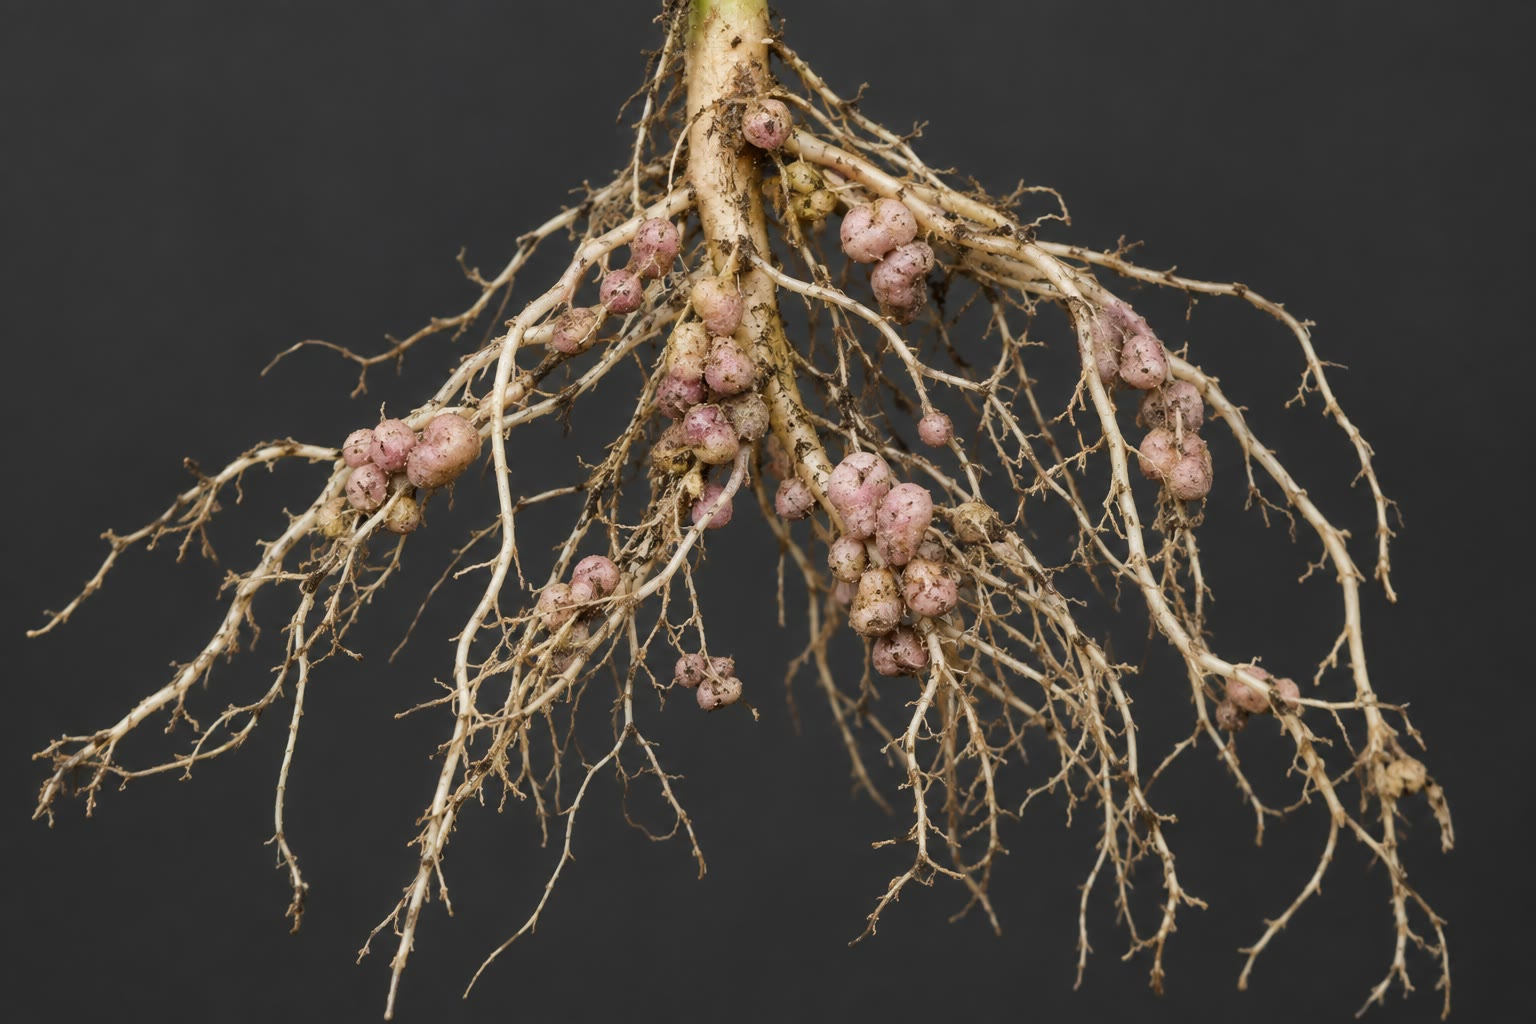
\includegraphics[width=0.44\linewidth]{images/book4/ai/b4-25-root-nodules.jpg}\hspace{0.04\linewidth}
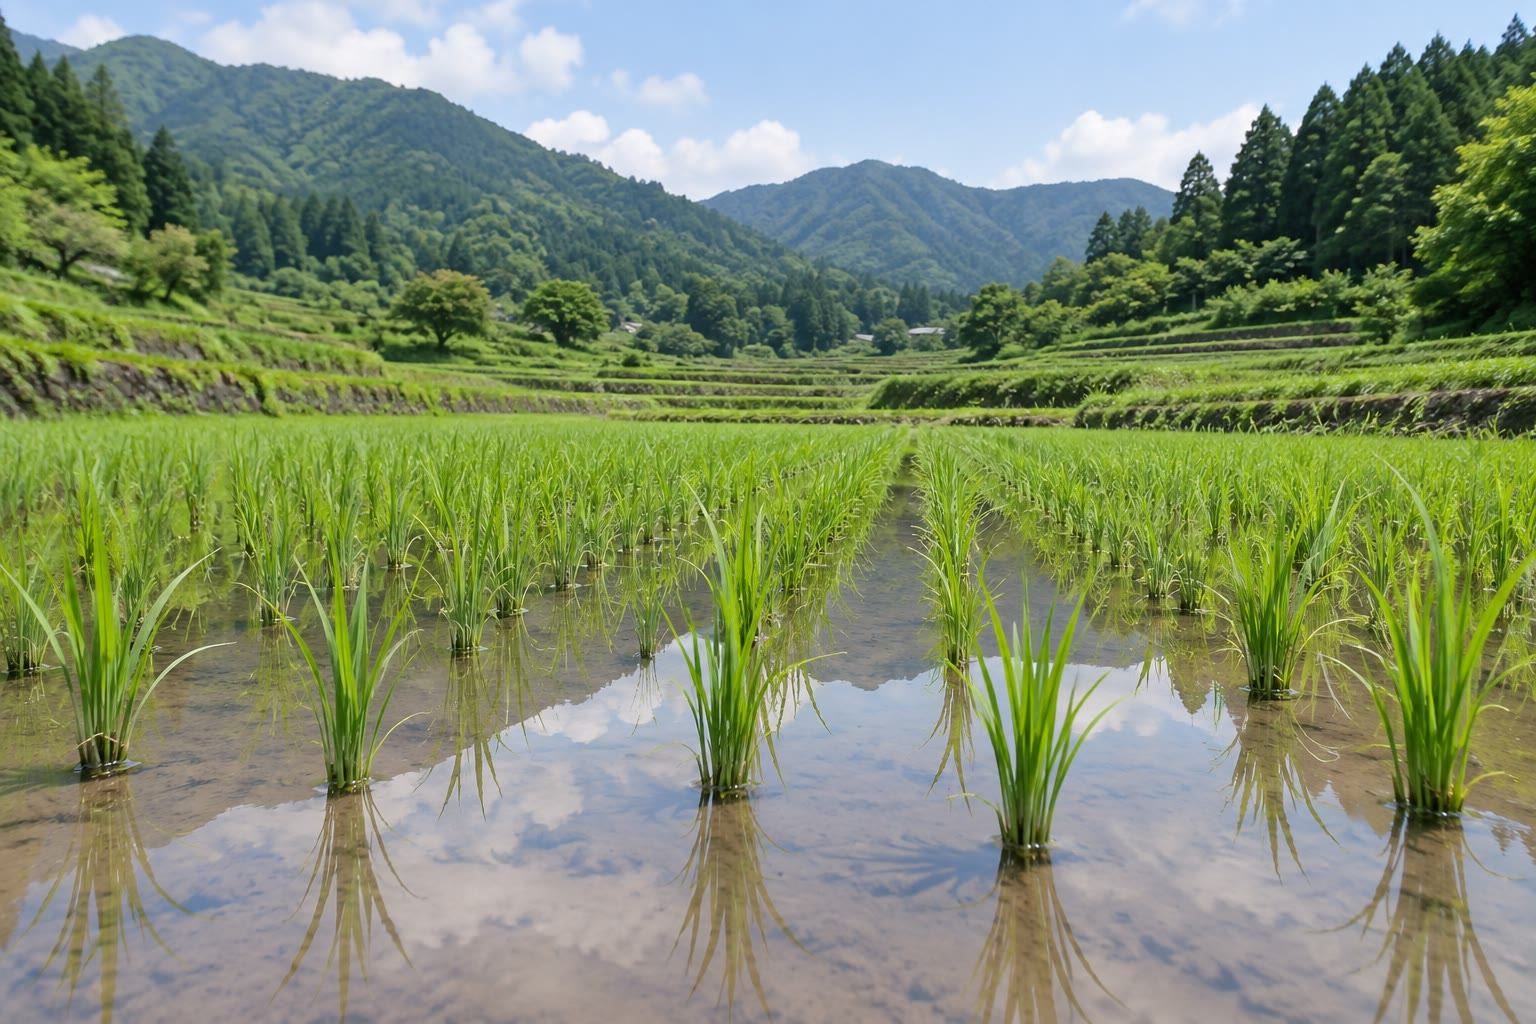
\includegraphics[width=0.44\linewidth]{images/book4/ai/b4-25-rice-paddy.jpg}

{\small Duas portas do \omterm{prop:b2:biogeochemical-cycles:nitrogen}{ciclo do nitrogênio}. À esquerda: nódulos
radiculares de uma leguminosa, cada um uma câmara em que rizóbios fixam
nitrogênio para seu hospedeiro. À direita: um arrozal inundado, anóxico
sob a superfície, onde a \omterm{def:b2:microbial-metabolism:anaerobic}{desnitrificação} devolve nitrogênio ao ar e os
metanogênicos produzem metano.}
\end{omfigure}

\section{O planeta perturbado}

\begin{example}[O que os números dizem]\label{ex:b2:biogeochemical-cycles:numbers}
Emissões de \qty{10}{GtC} por ano com uma \omterm{prop:b2:biogeochemical-cycles:carbon}{fração atmosférica} de
$0.45$ deixam \qty{4.5}{GtC}, ou \qty{2.1}{ppm}, no ar a cada ano ---
a inclinação observada. As emissões acumuladas desde 1850 são de cerca
de \qty{700}{GtC}, das quais \qty{290}{GtC} estão no ar (140~ppm), e o
restante no oceano e na terra. Para manter a atmosfera em qualquer
nível, as emissões líquidas devem cair ao que os sumidouros lentos ---
a mistura com o oceano profundo e o intemperismo, juntos abaixo de
\qty{1}{GtC} por ano --- conseguem absorver: a \emph{neutralidade
líquida} não é um slogan, mas a condição de \omterm{def:b2:biogeochemical-cycles:reservoir}{estado estacionário} do
\omterm{thm:b2:biogeochemical-cycles:box}{modelo de caixa} com um $\tau$ muito longo. Para o nitrogênio, a
duplicação do \omterm{def:b2:biogeochemical-cycles:reservoir}{fluxo} de nitrogênio fixado duplicou o nitrato dos rios,
produziu zonas mortas na foz do Mississippi e no Báltico, e elevou em um
quinto o $\mathrm{N_2O}$ da atmosfera, um gás de efeito estufa com \omterm{def:b2:biogeochemical-cycles:reservoir}{tempo
de residência} de um século. O \cref{ch:b2:global-change} acompanha as
consequências para os seres vivos.
\end{example}

\section{Exercícios}

\begin{exercise}[$\star$]\label{exo:b2:biogeochemical-cycles:1}
Defina \omterm{def:b2:biogeochemical-cycles:reservoir}{reservatório}, \omterm{def:b2:biogeochemical-cycles:reservoir}{fluxo} e \omterm{def:b2:biogeochemical-cycles:reservoir}{tempo de residência}, e calcule o \omterm{def:b2:biogeochemical-cycles:reservoir}{tempo de
residência} do carbono nas plantas terrestres (450 GtC, fotossíntese de
120 GtC por ano) e no oceano profundo (\num{37000} GtC, troca de cerca
de 100 GtC por ano).
\end{exercise}

\begin{exercise}[$\star$]\label{exo:b2:biogeochemical-cycles:2}
Converta \qty{2.5}{ppm} por ano em GtC, e \qty{10}{GtC} de emissões
em ppm.
\end{exercise}

\begin{exercise}[$\star$]\label{exo:b2:biogeochemical-cycles:3}
Nomeie os dois processos naturais que abrem o $\mathrm{N_2}$, o processo que
o devolve e as três etapas redox intermediárias, com os organismos
responsáveis.
\end{exercise}

\begin{exercise}[$\star$]\label{exo:b2:biogeochemical-cycles:4}
Por que o fósforo limita a produtividade mais vezes que o nitrogênio em
escala geológica, e o nitrogênio mais vezes que o fósforo numa dada
estação?
\end{exercise}

\begin{exercise}[$\star\star$]\label{exo:b2:biogeochemical-cycles:5}
Um lago de \qty{e7}{m^3} recebe \qty{2}{t} de fósforo por ano e renova
\qty{20}{\%} de sua água anualmente. Calcule sua concentração de
fósforo em \omterm{def:b2:biogeochemical-cycles:reservoir}{estado estacionário} e o tempo para atingir \qty{90}{\%}
dela depois que a entrada começa. E se a entrada for reduzida à metade?
\end{exercise}

\begin{exercise}[$\star\star$]\label{exo:b2:biogeochemical-cycles:6}
A partir dos dados de Keeling, calcule a taxa média de aumento do $\mathrm{CO_2}$ nos
anos 1960 (de 316 a \qty{325}{ppm} em dez anos) e nos anos 2010 (de 390
a 411 em nove anos), em ppm por ano e em GtC por ano.
\end{exercise}

\begin{exercise}[$\star\star$]\label{exo:b2:biogeochemical-cycles:7}
O dente de serra sazonal em Mauna Loa tem uma amplitude de cerca de
\qty{6}{ppm} entre pico e vale. Converta em GtC e compare com a produção
primária líquida anual das terras do hemisfério norte, cerca de
\qty{35}{GtC}. Por que o dente de serra é tão menor?
\end{exercise}

\begin{exercise}[$\star\star$]\label{exo:b2:biogeochemical-cycles:8}
A nitrogenase gasta 16 ATP por $\mathrm{N_2}$. Para uma leguminosa que fixa
\qty{200}{kg} de nitrogênio por hectare por ano, calcule os mols de
$\mathrm{N_2}$ fixados e o ATP gasto, e a massa de glicose que esse ATP
representa (cerca de 30 ATP por glicose). Que fração dos fotoassimilados
de uma cultura de \qty{10}{t/ha} isso representa?
\end{exercise}

\begin{exercise}[$\star\star$]\label{exo:b2:biogeochemical-cycles:9}
O plâncton cresce na razão de Redfield $\mathrm{C:N:P} = 106:16:1$.
A água do mar em profundidade contém \qty{2.2}{\micro mol/kg} de fosfato
e \qty{32}{\micro mol/kg} de nitrato. Qual se esgota primeiro quando uma
massa de água é trazida à superfície, e quanto carbono é fixado antes
disso?
\end{exercise}

\begin{exercise}[$\star\star\star$]\label{exo:b2:biogeochemical-cycles:10}
Trate a atmosfera como uma caixa com um excesso de carbono $E$ removido
à taxa $E/\tau$ pelos sumidouros e alimentado pelas emissões $Q$. Com $\tau =
50$ anos e $Q = \qty{10}{GtC/ano}$, qual é o excesso em \omterm{def:b2:biogeochemical-cycles:reservoir}{estado
estacionário} e a quantos ppm ele corresponde? Explique por que a
resposta real é pior.
\end{exercise}

\begin{exercise}[$\star\star\star$]\label{exo:b2:biogeochemical-cycles:11}
Os testes de bombas dobraram o $\mathrm{{}^{14}C}$ da atmosfera em 1963; o
excesso depois caiu pela metade a cada 11 anos, aproximadamente, embora o $\mathrm{{}^{14}C}$
tenha uma meia-vida de 5730 anos. Explique o que foi medido e o que
os 11 anos dizem sobre o \omterm{prop:b2:biogeochemical-cycles:carbon}{ciclo do carbono}.
\end{exercise}

\begin{exercise}[$\star\star\star$]\label{exo:b2:biogeochemical-cycles:12}
``Os seres humanos dobraram o \omterm{prop:b2:biogeochemical-cycles:nitrogen}{ciclo do nitrogênio} e apenas deram um
empurrãozinho no \omterm{prop:b2:biogeochemical-cycles:carbon}{ciclo do carbono}.'' Discuta com números: \omterm{def:b2:biogeochemical-cycles:reservoir}{fluxos}
fixados, frações do \omterm{def:b2:biogeochemical-cycles:reservoir}{fluxo} natural e \omterm{def:b2:biogeochemical-cycles:reservoir}{reservatórios} afetados.
\end{exercise}

\section{Problema: O balanço de carbono de um século}

\begin{problem}[{Problema de fim de semana --- um século de emissões
passado pelo modelo de caixa da atmosfera, a parte do oceano e a da
terra, a cascata do nitrogênio de um campo fertilizado a uma zona morta,
e o balanço de fósforo de um lago, terminando com a fração atmosférica,
a concentração atmosférica em 2100 e o nitrogênio perdido por
hectare}]
\label{pb:b2:biogeochemical-cycles:1}
Dados. Atmosfera em 1850: \qty{285}{ppm}; \qty{1}{ppm} $=
\qty{2.13}{GtC}$. Emissões acumuladas 1850--2020: \qty{700}{GtC};
$\mathrm{CO_2}$ atmosférico em 2020: \qty{412}{ppm}. Um campo de
\qty{1}{ha} recebe \qty{150}{kg} de fertilizante nitrogenado por ano;
a cultura absorve \qty{60}{\%}, \qty{25}{\%} são desnitrificados e o
restante é lixiviado. Um lago de \qty{5e7}{m^3} renova um décimo de sua
água por ano e recebe \qty{5}{t} de fósforo por ano.

\medskip
\noindent\textbf{Parte I --- A \omterm{prop:b2:biogeochemical-cycles:carbon}{fração atmosférica}.}
\begin{enumerate}
  \item Calcule o carbono atmosférico em 1850 e em 2020, e o
        aumento em GtC.
  \item Calcule a \omterm{prop:b2:biogeochemical-cycles:carbon}{fração atmosférica} ao longo de 1850--2020.
  \item Onde está o restante? Dê os dois sumidouros e, a partir da
        proposição, suas partes aproximadas.
  \item Se o oceano absorveu \qty{25}{\%} das emissões, em quanto seu
        carbono inorgânico dissolvido, \qty{38000}{GtC}, aumentou em
        termos relativos? Por que, apesar disso, o oceano superficial se
        acidifica de modo mensurável?
  \item Por que a \omterm{prop:b2:biogeochemical-cycles:carbon}{fração atmosférica} permanece mais ou menos constante
        enquanto as emissões crescem exponencialmente? (Considere o \omterm{thm:b2:biogeochemical-cycles:box}{modelo
        de caixa} com $Q \propto e^{t/T}$ e um sumidouro $E/\tau$.)
  \item Qual seria a \omterm{prop:b2:biogeochemical-cycles:carbon}{fração atmosférica} se as emissões fossem
        mantidas constantes durante muitos séculos?
\end{enumerate}

\medskip
\noindent\textbf{Parte II --- O século que vem.}
Modele o excesso de carbono $E$ (acima do nível de 1850) com
$\mathrm{d}E/\mathrm{d}t = Q - E/\tau$, $\tau = 100$ anos.
\begin{enumerate}[resume]
  \item Calcule o excesso em 2020, em GtC.
  \item Com $Q$ mantido em \qty{10}{GtC/ano}, calcule o excesso em \omterm{def:b2:biogeochemical-cycles:reservoir}{estado
        estacionário} e a concentração que ele implica.
  \item Resolva para $E(t)$ a partir de 2020 com $Q = 10$ e dê $E$ em
        2100 e a concentração.
  \item Agora faça $Q$ cair linearmente até zero entre 2020 e 2070 e
        permanecer em zero. Calcule $E$ em 2070 (integre a equação;
        a solução particular para um $Q$ linear é linear mais uma
        constante) e em 2100.
  \item Compare as duas concentrações em 2100.
  \item Por que um único $\tau$ é otimista para o segundo cenário?
\end{enumerate}

\medskip
\noindent\textbf{Parte III --- A cascata do nitrogênio.}
\begin{enumerate}[resume]
  \item Calcule o nitrogênio absorvido pela cultura, desnitrificado e
        lixiviado, por hectare por ano.
  \item O nitrogênio lixiviado chega a um rio como nitrato e depois ao
        mar, onde o plâncton o usa na razão de Redfield. Quanto
        carbono ele permite ao plâncton fixar?
  \item Esse carbono afunda e é respirado em profundidade, consumindo
        oxigênio à razão de 1 $\mathrm{O_2}$ por C. Calcule o oxigênio consumido, em
        mols e em quilogramas.
  \item Um metro cúbico de água do mar contém cerca de \qty{0.25}{mol} de
        $\mathrm{O_2}$ quando saturado. Quantos metros cúbicos de água de fundo
        a lixiviação de um hectare desoxigena?
  \item A fração desnitrificada escapa em parte como $\mathrm{N_2O}$,
        \qty{1}{\%} do nitrogênio desnitrificado. Calcule o $\mathrm{N_2O}$
        por hectare por ano e seu equivalente de aquecimento em $\mathrm{CO_2}$
        (o $\mathrm{N_2O}$ vale 270 vezes o $\mathrm{CO_2}$ por quilograma).
  \item Compare com o $\mathrm{CO_2}$ emitido para produzir o fertilizante
        (cerca de \qty{4}{kg} de $\mathrm{CO_2}$ por quilograma de nitrogênio
        pelo \omterm{prop:b2:biogeochemical-cycles:nitrogen}{processo Haber--Bosch}).
\end{enumerate}

\medskip
\noindent\textbf{Parte IV --- O lago.}
\begin{enumerate}[resume]
  \item Calcule o \omterm{def:b2:biogeochemical-cycles:reservoir}{tempo de residência} do fósforo no lago se a única
        perda for a renovação da água, e sua concentração em \omterm{def:b2:biogeochemical-cycles:reservoir}{estado
        estacionário} em \unit{mg/m^3}.
  \item Os lagos com mais de \qty{30}{mg/m^3} de fósforo são
        eutróficos. Este é?
  \item A sedimentação remove fósforo com sua própria constante de tempo
        de 5 anos. Recalcule o \omterm{def:b2:biogeochemical-cycles:reservoir}{tempo de residência} e a
        concentração.
  \item A entrada é reduzida a \qty{1}{t} por ano. Calcule o novo
        \omterm{def:b2:biogeochemical-cycles:reservoir}{estado estacionário} e o tempo para chegar a menos de \qty{10}{\%} dele.
  \item Por que muitos lagos se recuperam mais lentamente do que este
        cálculo prevê?
  \item Calcule o carbono que o fósforo do lago pode incorporar ao
        plâncton a cada ano, na razão de Redfield, a partir da entrada de
        \qty{5}{t}.
  \item Enuncie o resultado: a \omterm{prop:b2:biogeochemical-cycles:carbon}{fração atmosférica}, as duas
        concentrações em 2100 e o nitrogênio lixiviado por
        hectare.
\end{enumerate}
\end{problem}
